\documentclass[12pt]{article}
\usepackage{iftex}
\usepackage{graphicx}
\usepackage{enumitem}
\usepackage{hyperref}
\usepackage[style=apa, backend=biber]{biblatex}
\addbibresource{phd_bombus.bib}
\setcounter{maxnames}{20}
\setcounter{minnames}{1}
\usepackage{color}
\usepackage{amsmath}
\usepackage{amssymb}
\usepackage[export]{adjustbox}
\usepackage{verbatim}
\usepackage{mathpazo}
\usepackage{setspace}
\usepackage{multirow}
\usepackage{lscape}
\usepackage{fancyhdr}
\usepackage[normalem]{ulem}
\usepackage{rotating}
\usepackage{chngcntr}
\usepackage{float}
\usepackage[parfill]{parskip}
\usepackage[tiny,compact]{titlesec}
\usepackage{longtable}
\usepackage{textcomp}
\usepackage{rotating}
\usepackage{xr}
\usepackage{caption}
\usepackage{siunitx}
\usepackage[T1]{fontenc}
\usepackage{gensymb}
\sisetup{round-mode=places, round-precision=2, detect-all}

\newcommand{\flagged}[1] {
  \textcolor{blue}{#1}
}

\hypersetup{colorlinks=true, linkcolor=black, citecolor=black}
\RequirePackage{lineno}

\renewcommand{\thefigure}{A\arabic{figure}}  % Prefix figures with "S"
\setcounter{figure}{0}  % Reset figure counter
\renewcommand{\thetable}{A\arabic{table}}
\setcounter{table}{0}
\setcounter{section}{0}

\def\title{Appendix 1 -- Population Genetics and Colony Assignments}



\begin{document}
\begin{center}
  {\large \title \par}
\end{center}\par

\section{Assessing locus $F_{is}$, $F_{st}$ and linkage disequilibrium}

\begin{figure}[H]
    \centering
    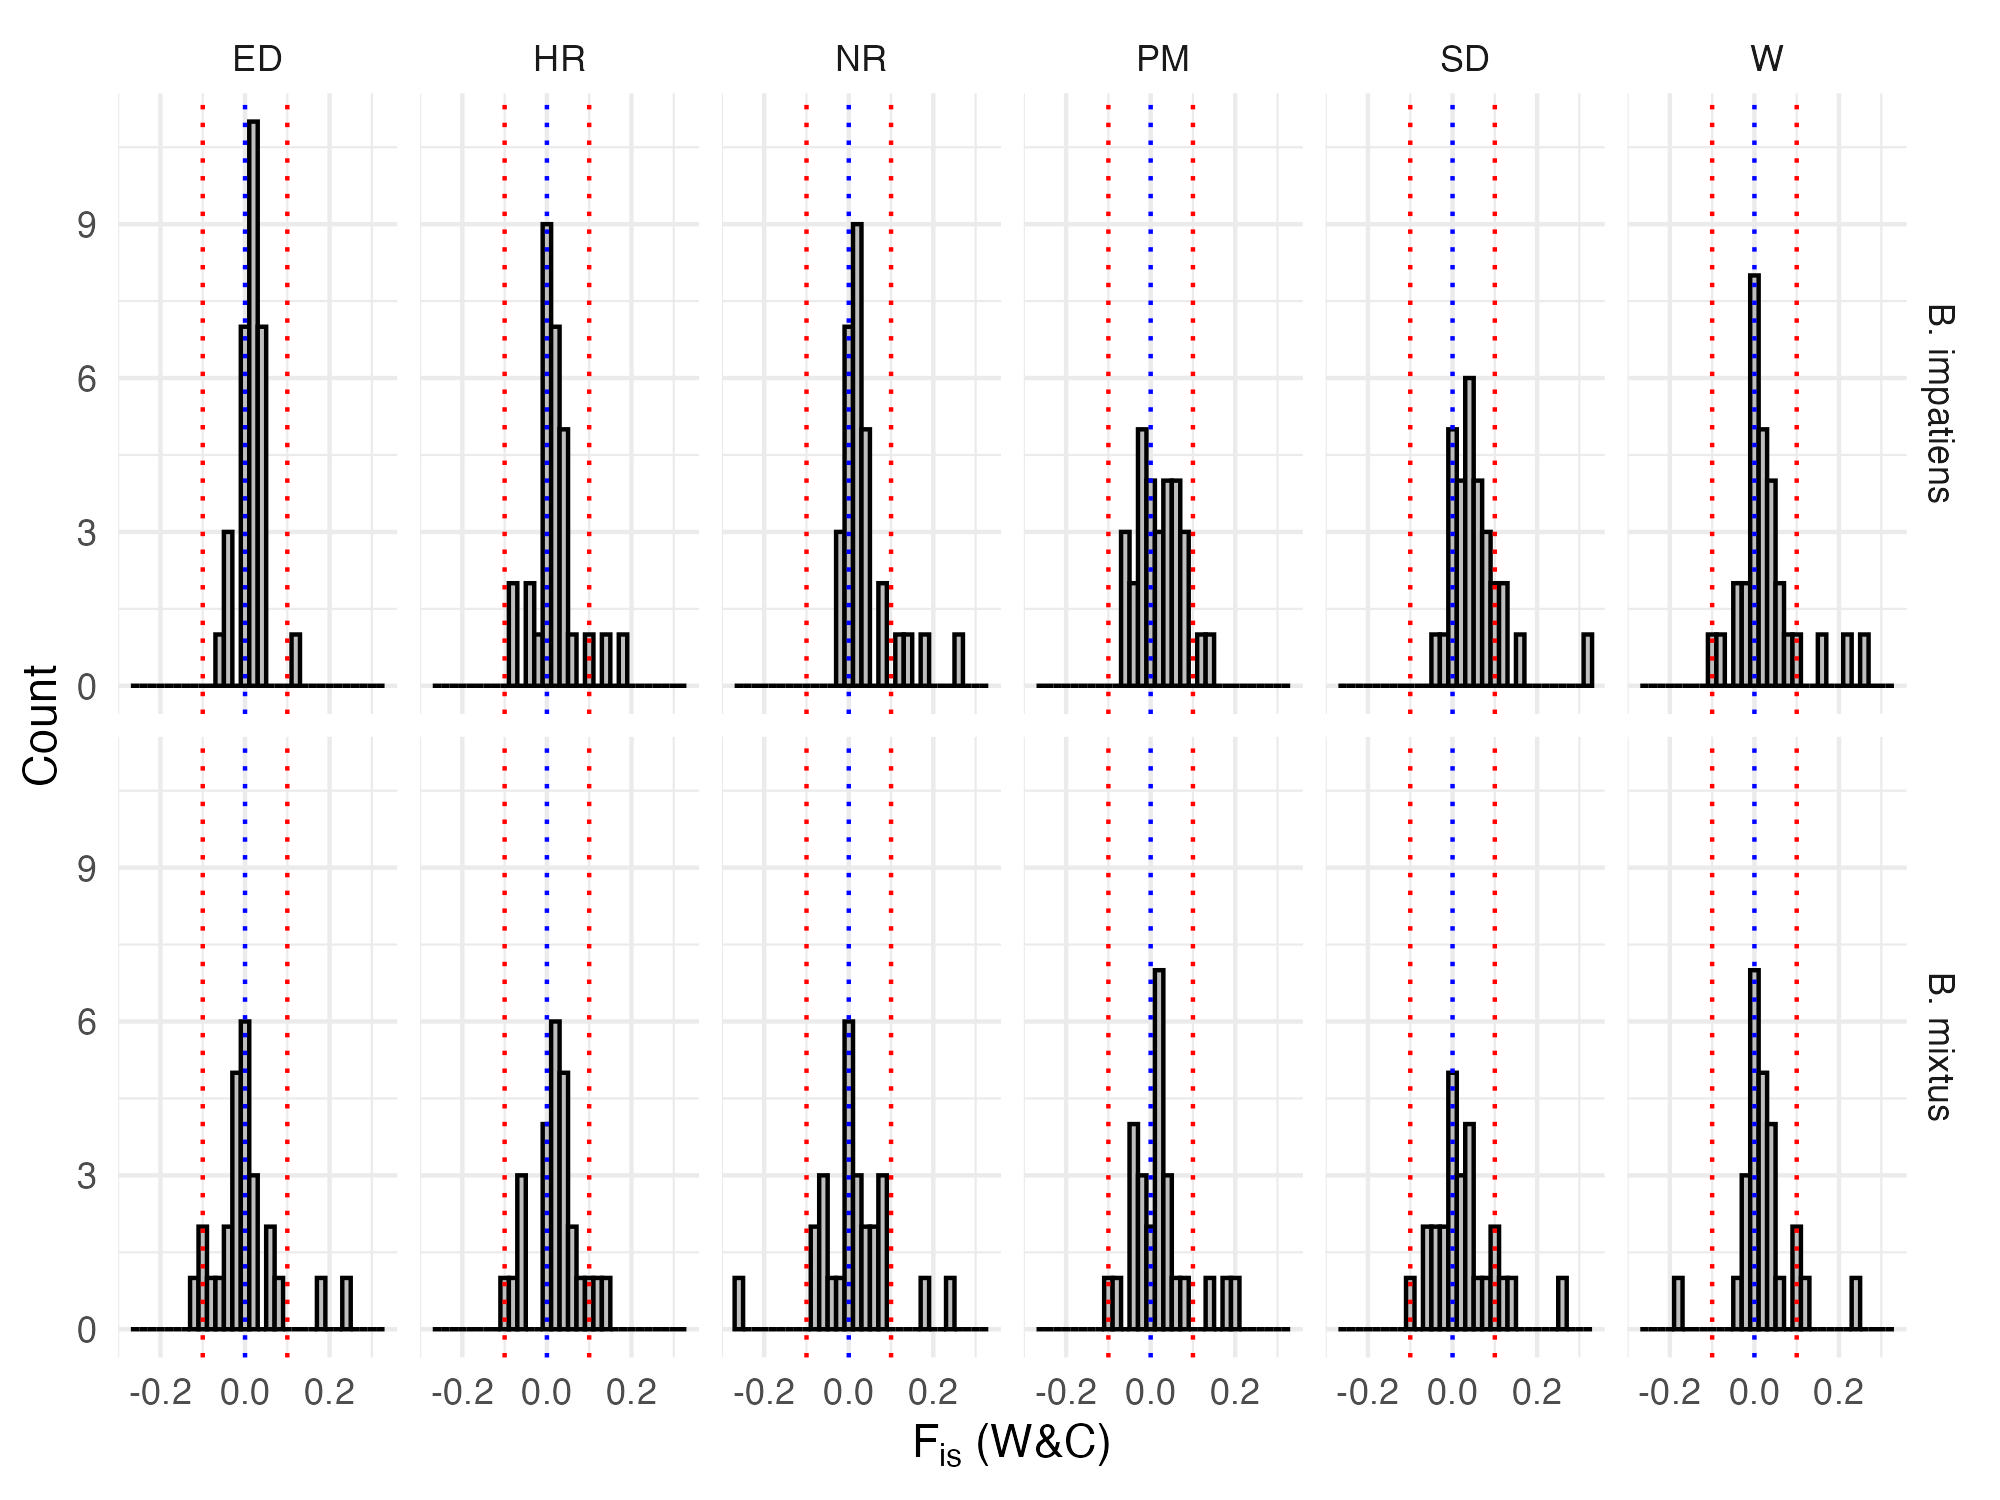
\includegraphics[width=\linewidth]{appendix_figures/Fis.jpg}
    \caption{Estimates of $F_{is}$ for each locus in each subpopulation. Estimates from 2022 and 2023 were calculated separately but are shown together for each site x species combination. Blue dotted lines indicates $F_{is} = 0$ and red dotted lines indicate $F_{is} = \pm 0.1$.}
    \label{fig:Fis}
\end{figure}


\begin{figure}[H]
    \centering
    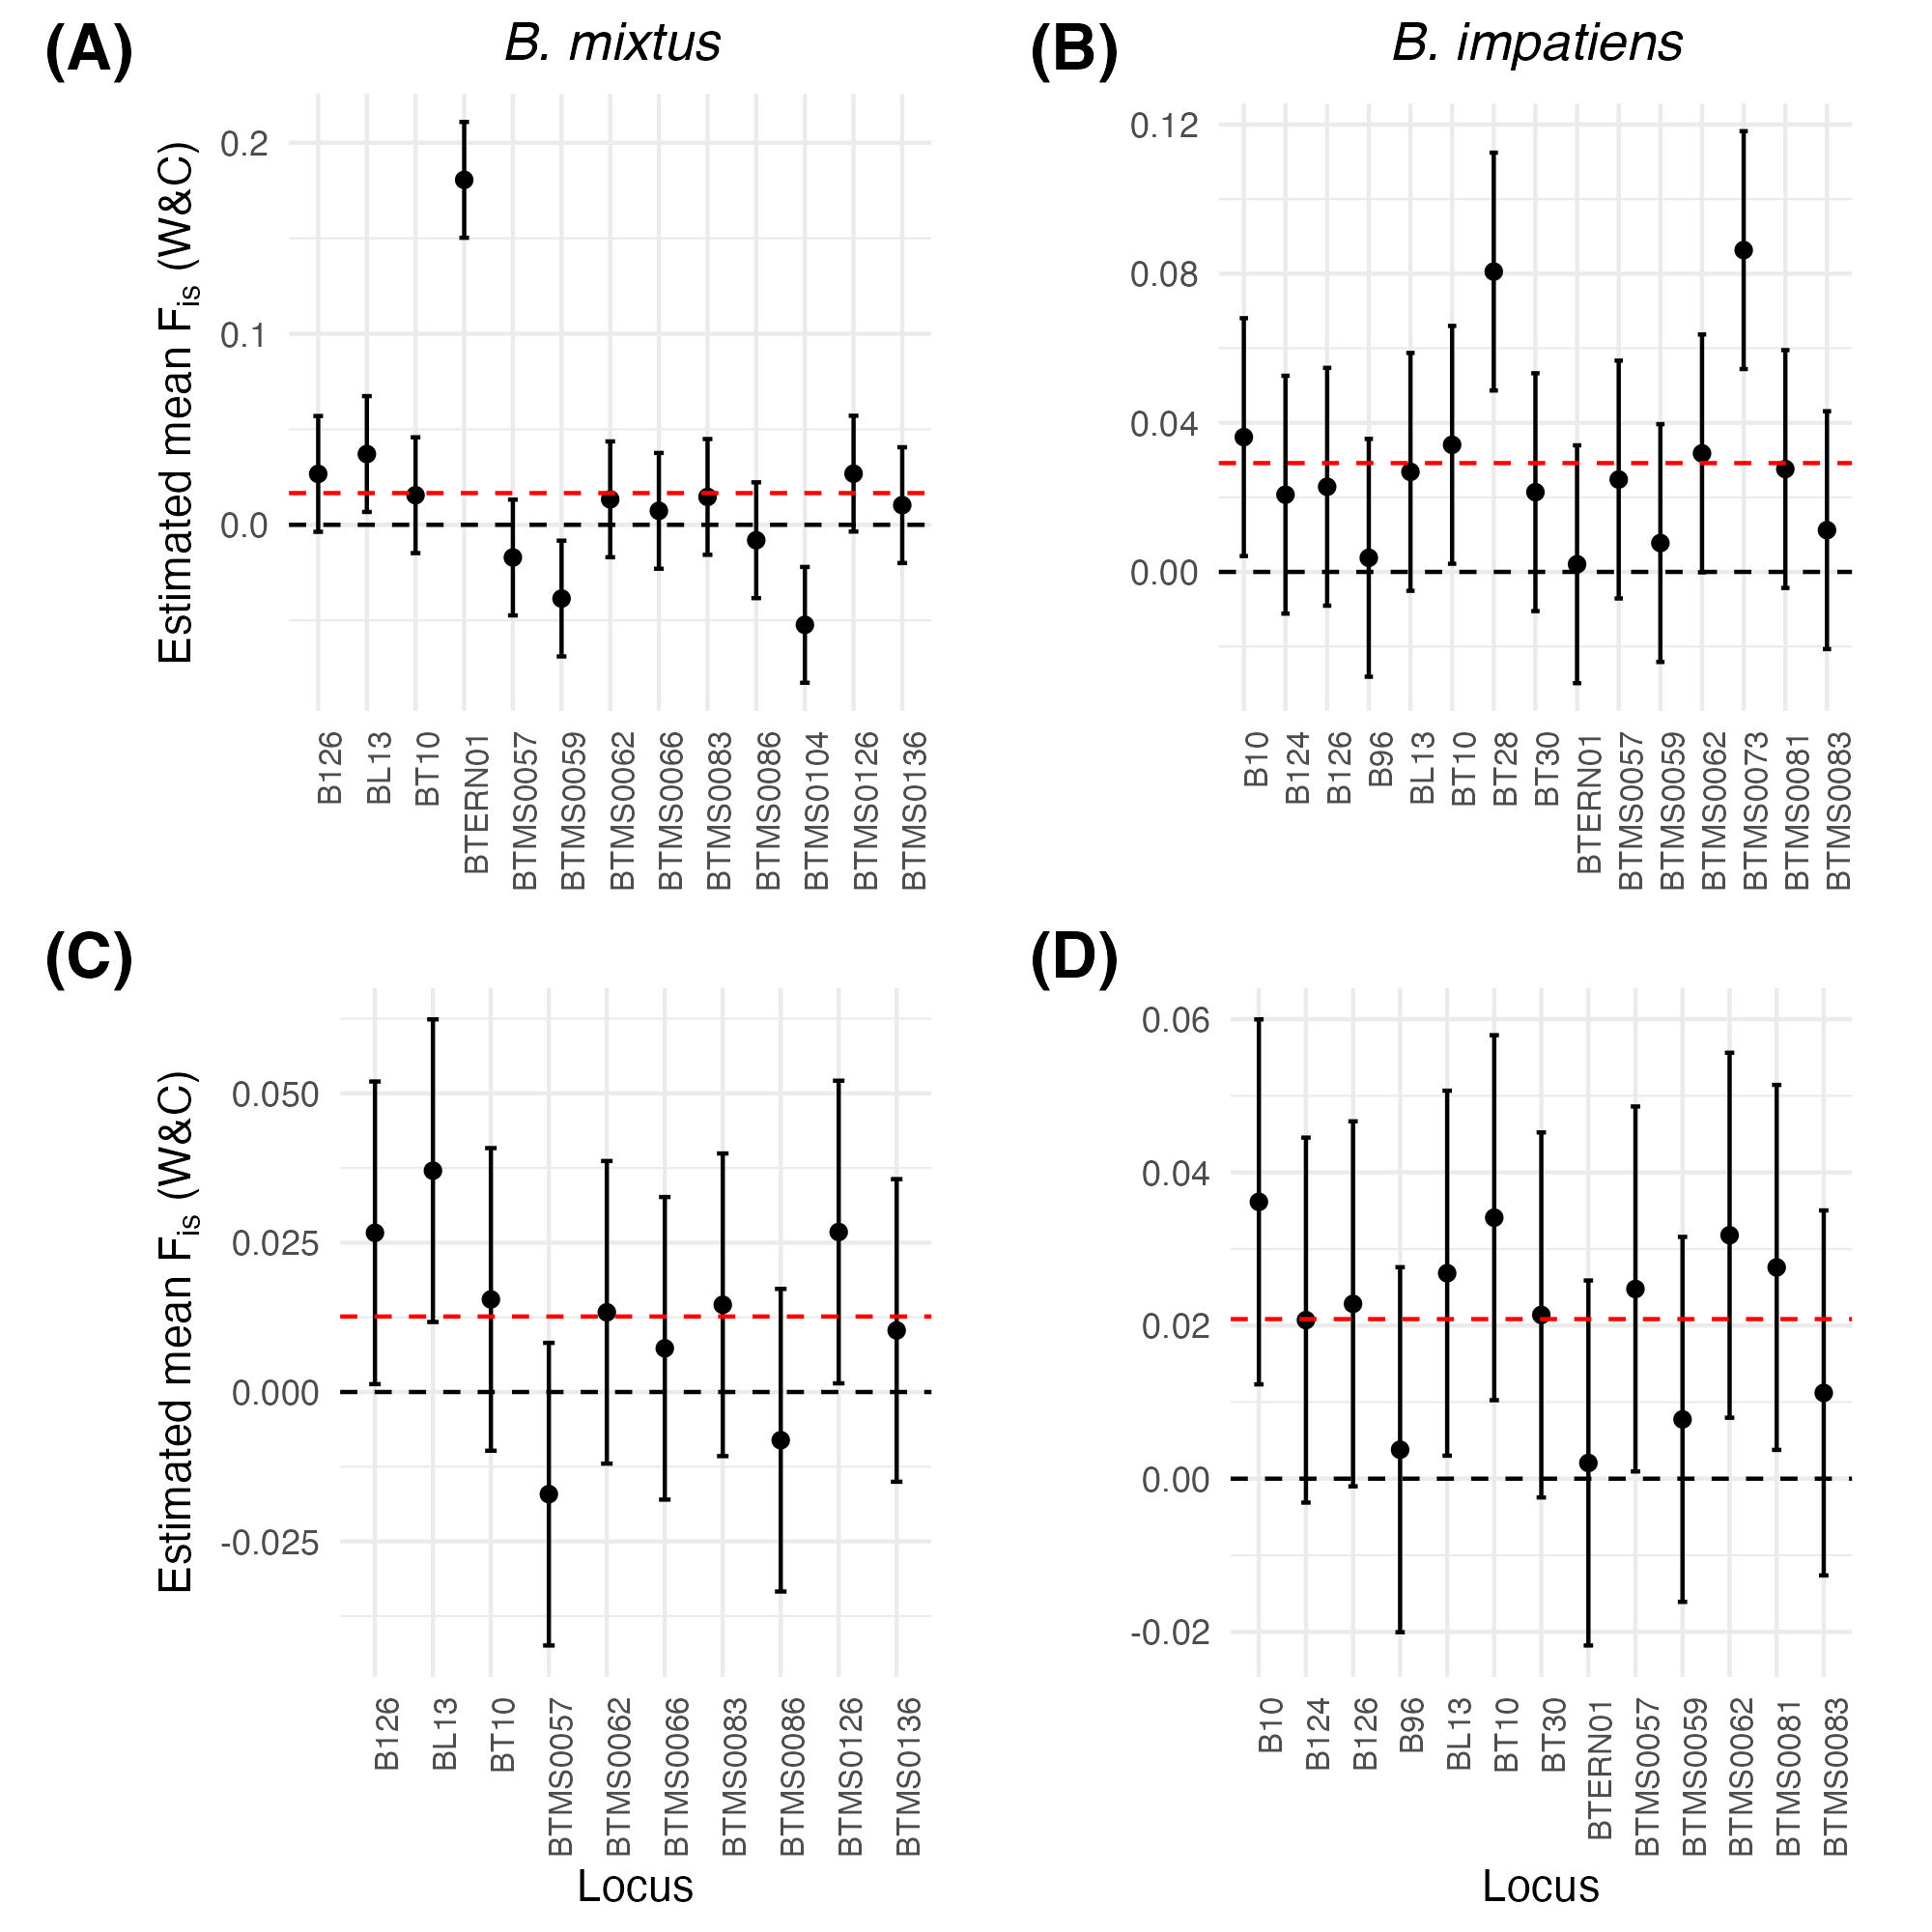
\includegraphics[width=\linewidth]{appendix_figures/marginalmeans.jpg}
    \caption{Locus-specific $F_{is}$ marginal means. A) \emph{B. mixtus} all loci; B) \emph{B. impatiens} all loci; C) \emph{B. mixtus} loci following iterative removal of loci which differed significantly from global mean $F_{is}$; D) \emph{B. impatiens} loci following iterative removal of loci which differed significantly from global mean $F_{is}$. Dashed black line denotes $F_{is} = 0$, dashed red line denotes global mean $F_{is}$ for each species.}
    \label{fig:marginalmeans}
\end{figure}


\begin{figure}[H]
    \centering
    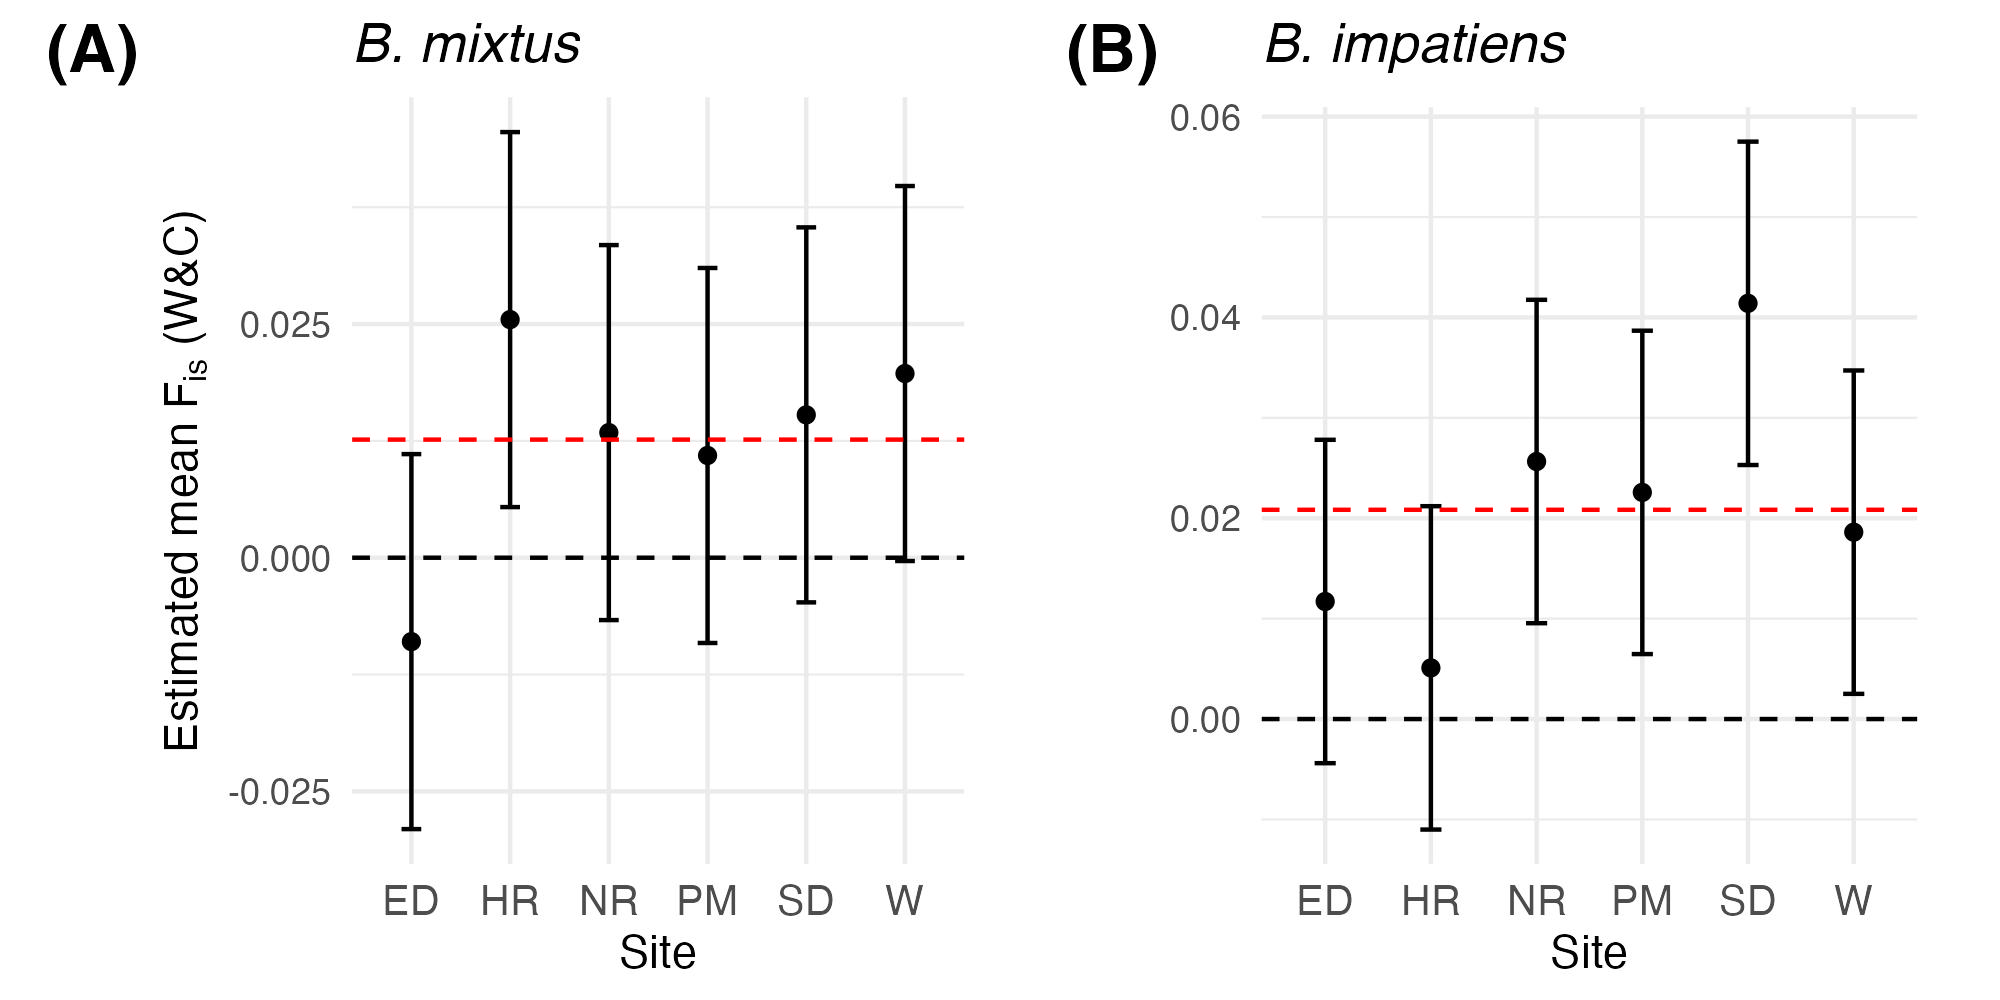
\includegraphics[width=\linewidth]{appendix_figures/siteFis.jpg}
    \caption{Site-specific $F_{is}$ marginal means following removal of low-quality loci for A) \emph{B. mixtus} and B) \emph{B. impatiens}. Dashed black line denotes $F_{is} = 0$, dashed red line denotes global mean $F_{is}$ for each species.}
    \label{fig:siteFis}
\end{figure}


\section{Testing COLONY on simulated data}
To test the informativeness of our genetic loci and to validate the accuracy of COLONY2.0 \parencite{jonesCOLONYProgramParentage2010} for accurately detecting siblingships amongst our samples, we performed simulations using realistic family size distributions and the allelic frequencies present in our real data.

We approached this simulations with four objectives:

(i) To determine false positive and false negative siblingship assignment rates, given the informativeness of our microsatellite datasets, 

(ii) To inform an appropriate strategy (probability threshold, number of runs of the software) for maintaining or rejecting each sib-pair;

(iii) To select suitable software parameters, and in particular to evaluate the usefulness of siblingship size priors and exclusion of across-site siblingships for reducing false positive rates as sample size increases;

(iv) To assess whether modelling female polygamy would improve family reconstruction in the case of sibling genotypes simulated under varying rates of multiple paternity.

\subsection{Simulation strategy}

\subsubsection{Spatially explicit siblingships}
We first simulated spatially explicit siblingships following \textcite{popeInferringForagingRanges2017}. We began by simulating six 5 x 5 trapping grids (locations $k \in \kappa$) on a single raster surface comprised of cells $j \in \mathbb{J}$. Colonies ($i \in \mathbb{C}$) were distributed uniformly at random throughout the ``landscape."

We sampled individuals from colonies $i \in \mathbb{C}$ captured at traps $k \in \mathbb{K}$ from the joint distribution $\Pr(s, c \mid s \in \kappa)$, where $\{s,c\}$ are the indices of a random visitation event of an individual from colony $c \in \mathbb{C}$ to grid cell $s \in \mathbb{J}$.

To do this, we first sampled a trap ($k$) from

\[
\Pr(s = k \mid s \in \kappa) \;=\; \frac{\Pr(s = k)}{\Pr(s \in \kappa)} \tag{1}
\]

where

\[
\Pr(s = k) \;=\; \sum_{i \in C} \Pr(s = k \mid c = i)\,\Pr(c = i)
\]

and

\[
\Pr(s \in \kappa) \;=\; \sum_{i \in \mathbb{C}} \Pr(s \in \kappa \mid c = i)\,\Pr(c = i)
                  \;=\; \sum_{i \in \mathbb{C}} \sum_{k \in \kappa} \Pr(s = k \mid c = i)\,\Pr(c = i)
\]

Combining these statements gives a probability of sampling from trap $k$ of:

\[
\Pr(s = k \mid s \in \kappa) \;=\; \frac{\sum_{i \in C} \Pr(s = k \mid c = i)\,\Pr(c = i)}{\sum_{i \in \mathbb{C}} \sum_{k \in \kappa} \Pr(s = k \mid c = i)\,\Pr(c = i)} \tag{2}
\]

We then sampled a colony ($i$) from

\[
\Pr(c = i \mid s = k) \;=\; \frac{\Pr(s = k \mid c = i) \Pr(c = i)}{\Pr(s = k)} \;=\; \frac{\Pr(s = k \mid c = i) \Pr(c = i)}{\sum_{i \in \mathbb{C}} \Pr(s = k \mid c = i)\,\Pr(c = i)} \tag{3}
\]


We define the foraging kernel of workers from colony $i$ as:

\[
\Pr(s = k \mid c = i)
\;=\; 
\frac{\lambda_i(k)}{\sum_{j \in J} \lambda_i(j)} \tag{4}
\]

The visitation intensity of individuals from colony $i$ to location $j$ is defined as: 

\[
ln(\lambda_i(j)) = \frac{- \lVert x_j - \delta_i \rVert}{\rho} \tag{5}
\]

where $x_j$ are the spatial coordinates of any grid cell in the raster, and $\delta_i$ are the spatial coordinates of colony $i$. The foraging kernel in this example is therefore assumed to be symmetrical and exponentially decaying as a function of distance from the colony location. This means that the total visitation of each colony across the landscape ($\sum_{j \in J} \lambda_i(j)$) is the same for all colonies, and can be represented using the constant $\mathbb{D}$. $\Pr(c = i)$ is the proportion of all bees in the landscape originating from colony $i$, e.g., $\Pr(c = i) = \frac{n_i}{N}$ where $n_i$ is the number of bees from colony $i$, and $N = \sum_{i \in \mathbb{C}} n_i$ is the total number of bees in the landscape.

Combining (4) with (2) and (3) gives the probability of sampling an individual from trap $k$

% with variable foraging kernels
%\[
%\Pr(s = k \mid s \in \kappa) \;=\; \frac{\sum_{i \in \mathbb{C}} \frac{\lambda_i(k)}{\sum_{j \in %J} \lambda_i(j)}\,\frac{n_i}{N}}{\sum_{k \in \kappa} \sum_{i \in \mathbb{C}} \frac{\lambda_i(k%)}{\sum_{j \in J} \lambda_i(j)}\,\frac{n_i}{N}}
%\]

% with identical foraging kernels
\[
\Pr(s = k \mid s \in \kappa) \;=\; \frac{\sum_{i \in \mathbb{C}} \lambda_i(k) \frac{n_i}{N}}{\sum_{k \in \kappa} \sum_{i \in \mathbb{C}} \lambda_i(k) \frac{n_i}{N}}
\]

and the probability that the individual originates from colony $i$

% with variable foraging kernels
% \[
% \Pr(c = i \mid s = k) \;=\;  \frac{\frac{\lambda_i(k)}{\sum_{j \in J} \lambda_i(j)} \frac{n_i}{N}}{\sum_{i \in \mathbb{C}} \frac{\lambda_i(k)}{\sum_{j \in J} \lambda_i(j)} \frac{n_i}{N}}
% \]

% with identical foraging kernels
\[
\Pr(c = i \mid s = k) \;=\; \frac{\lambda_i(k) \frac{n_i}{N}}{\sum_{i \in \mathbb{C}} \lambda_i(k) \frac{n_i}{N}}
\]

For each simulation, samples are drawn from $\Pr(s, c \mid s \in \kappa)$ until a stopping point (desired number of samples) is reached. $n_i$ is updated after each "sampling event" to prevent oversampling from colonies located very close to traps.

To verify that the size of sampled siblingships (e.g., number of siblings per sibling group) accurately mirrors the distribution of siblingship sizes in real data, we compared our simulated distributions to the distribution of siblingshp sizes in our real data (\ref{fig:sibshipsizedist}). For this simulation strategy, we found that moderating the background density of colonies (i.e., the total number of colonies simulated on the landscape) was the most effective strategy for controlling average siblingship size. A larger number of simulated colonies resulted in a higher proportion of singleton colonies (colonies represented by only a single individual).

%%%%%%% INSERT SIBSHIP SIZE DISTRIBUTION FIGURE HERE!!!! %%%%%%%%%%%%%


\subsubsection{Multilocus genotypes}
We simulated multilocus genotypes for each sampled individual under several mating scenarios. In the simplest case, we assume monogamy for both males and queens. The majority of the simulation results presented below follow this assumption. In a second set of simulations, we assumed varying rates of polyandry (e.g., queen polygamy) to assess the impact of this assumption on siblingship inferences. For each simulation we used the following heuristic:

(i) Simulate parental genotypes for each siblingship based on the allele frequencies present in our real data;

(ii) Randomly draw offspring genotypes from the set of possible parental alleles at each locus.

This method allows us to draw conclusions based on the informativeness of our specific genetic datasets, rather than based on an idealized situation with perfect data. We performed simulations based on allele frequencies for both species (\emph{B. mixtus} and \emph{B. impatiens}) because variation in marker number and/or polymorphic information content could lead to differing results. We inferred allele frequencies from an earlier run of COLONY version 2.0.6.5, which accounts for heightened frequency of alleles present in large families; because average family size was small in our dataset (< 2 individuals) and large families were rare (Fig \ref{fig:sibdistribution}), raw allele frequencies would have likely been sufficient.

For simulations involving monogamous mating, male genotypes were assigned directly to all offspring in the siblingship; in families which were assigned multiple paternity, we assumed two fathers and assigned inheritance of paternal multilocus genotypes from $\Pr(father_1, father_2) = (0.7, 0.3)$ following the proportions observed for \emph{B. impatiens} in \textcite{birdMatingFrequencyEstimation2024}.

After assigning a multilocus genotype to each individual, we introduced errors and data missingness based on observed rates for our real datasets. To introduce errors, we mutated each allele with a probability equal to the rate of errors for that locus and species; we assumed that most errors would be due to contamination, rather than allele dropout, and drew new (erroneous) alleles from the allele frequency distribution for each species. We observed that individuals which were missing data for \emph{one} copy of a locus were more likely to be missing data for \emph{both} copies than if missingness were distributed uniformly at random. This is likely because there were two primary missingness-generating processes in real data: amplification failure (both alleles missing for an individual) and binning failure (one or both alleles missing for an individual). (In cases were only one copy of a locus failed to amplify, heterozygous individuals would be falsely classified as homozygous---an error, rather than missing data). To mimic the observed distribution of missingness, we first calculated the proportion of missing data for each marker ($P_{missing}$) and then removed data for (i) both alleles of each individual with probability $1/3 * P_{missing}$ and for (ii) a single allele per individual with probability $1/3 * P_{missing}$.

\subsection{Determining an appropriate heuristic for maintaining or rejecting inferred siblingships}

Like any family reconstruction software, COLONY is known to produce some errors. Most concerningly (in our case), improper specification of the program can lead ot a high number of inferred siblingships between non-siblings, referred to hereafter as \emph{false positive sibships}. Our own preliminary data analyses resulted in a high number of inferred siblingships between individuals separated by >20 km when individuals from all study sites were permitted to form siblingships. While the biology of bumblebee foraging/dispersal does not unilaterally exclude the possibility of such distant relationships, the likelihood of observing such separation distances is extremely small, and unlikely to represent biological reality except in very rare cases (see discussion below, section "Observing colonymates at multiple sites").

A common strategy in the \emph{Bombus} colony assignment literature is to repeat multiple "runs" (usually 2-5) of the COLONY software on each dataset, and maintain family groups which are inferred in all runs at or above some confidence threshhold (usually $P \ge 0.95$, but sometimes $P \ge 0.8$). See, for example, \textcite{carvellMolecularSpatialAnalyses2012, raoBumbleBeeHymenoptera2012, dreierFinescaleSpatialGenetic2014a, geibBumbleBeeNest2015a, carvellBumblebeeFamilyLineage2017a, molaWildfireRevealsTransient2020a}. However, we are not aware of any studies which give support for a particular threshhold probability or number of runs necessary to reach a particular confidence level in assignments, nor to achieve a satisfactory balance between false positive siblingships and missed (false negative) siblingships. Indeed, the desireable threshhold is likely to vary as a function of the number and informativeness of markers for a given population.

To overcome these limitations, we tested probability exclusion criteria from $P = 0.95$ to $P = 1$, for 1 or 5 runs of COLONY version 2.0.6.5. Further, we compared the use of family cluster probabilities (COLONY output file .BestCluster---hereafter referred to as the family method) and full sibling dyad probabilities (COLONY output .FullSibDyad---hereafter referred to as the dyad method).

We began by simulating 5 datasets (e.g., different siblingship arrangements with unique parental genotypes) consisting of n = 1200 individuals each, which was roughly the midpoint of population sizes for our real data. For each dataset we performed 5 runs of COLONY (see Table \ref{tab:simulationspecs} for a summary of COLONY software settings).

Based on our results, we conclude that the software converges reliably for datasets like ours, and that repeated runs of the software have litte or no effect on conclusions drawn. In most cases, false positive and false negative rates are either identical or nearly overlapping, regardless of the numbers of runs (Fig \ref{fig:fpr_repetition, fig:fnr_repetition}). We therefore recommend that to save time and computational resources, researchers should check for convergence for each microsatellite dataset using 2-3 runs of the software, and if convergence is achieved they should feel confident that a single run is sufficient to identify siblingships.

For both species we found that increasing the probability threshhold from 0.95 to 1 resulted in a greater reduction of false positives for the dyad method than for the family method; in general, a probability threshold $\ge$ 0.99 was necessary to maintain false positive rates at around 5\%. For $P = 1$ the dyad method led to a higher proportion of false negatives ($\ge 5\%$) \ref{fig:fnr_repetition}. For this reason, we would not recommend this stringent a threshold unless a very low rate of false positives is required.

\begin{figure}[H]
    \centering
    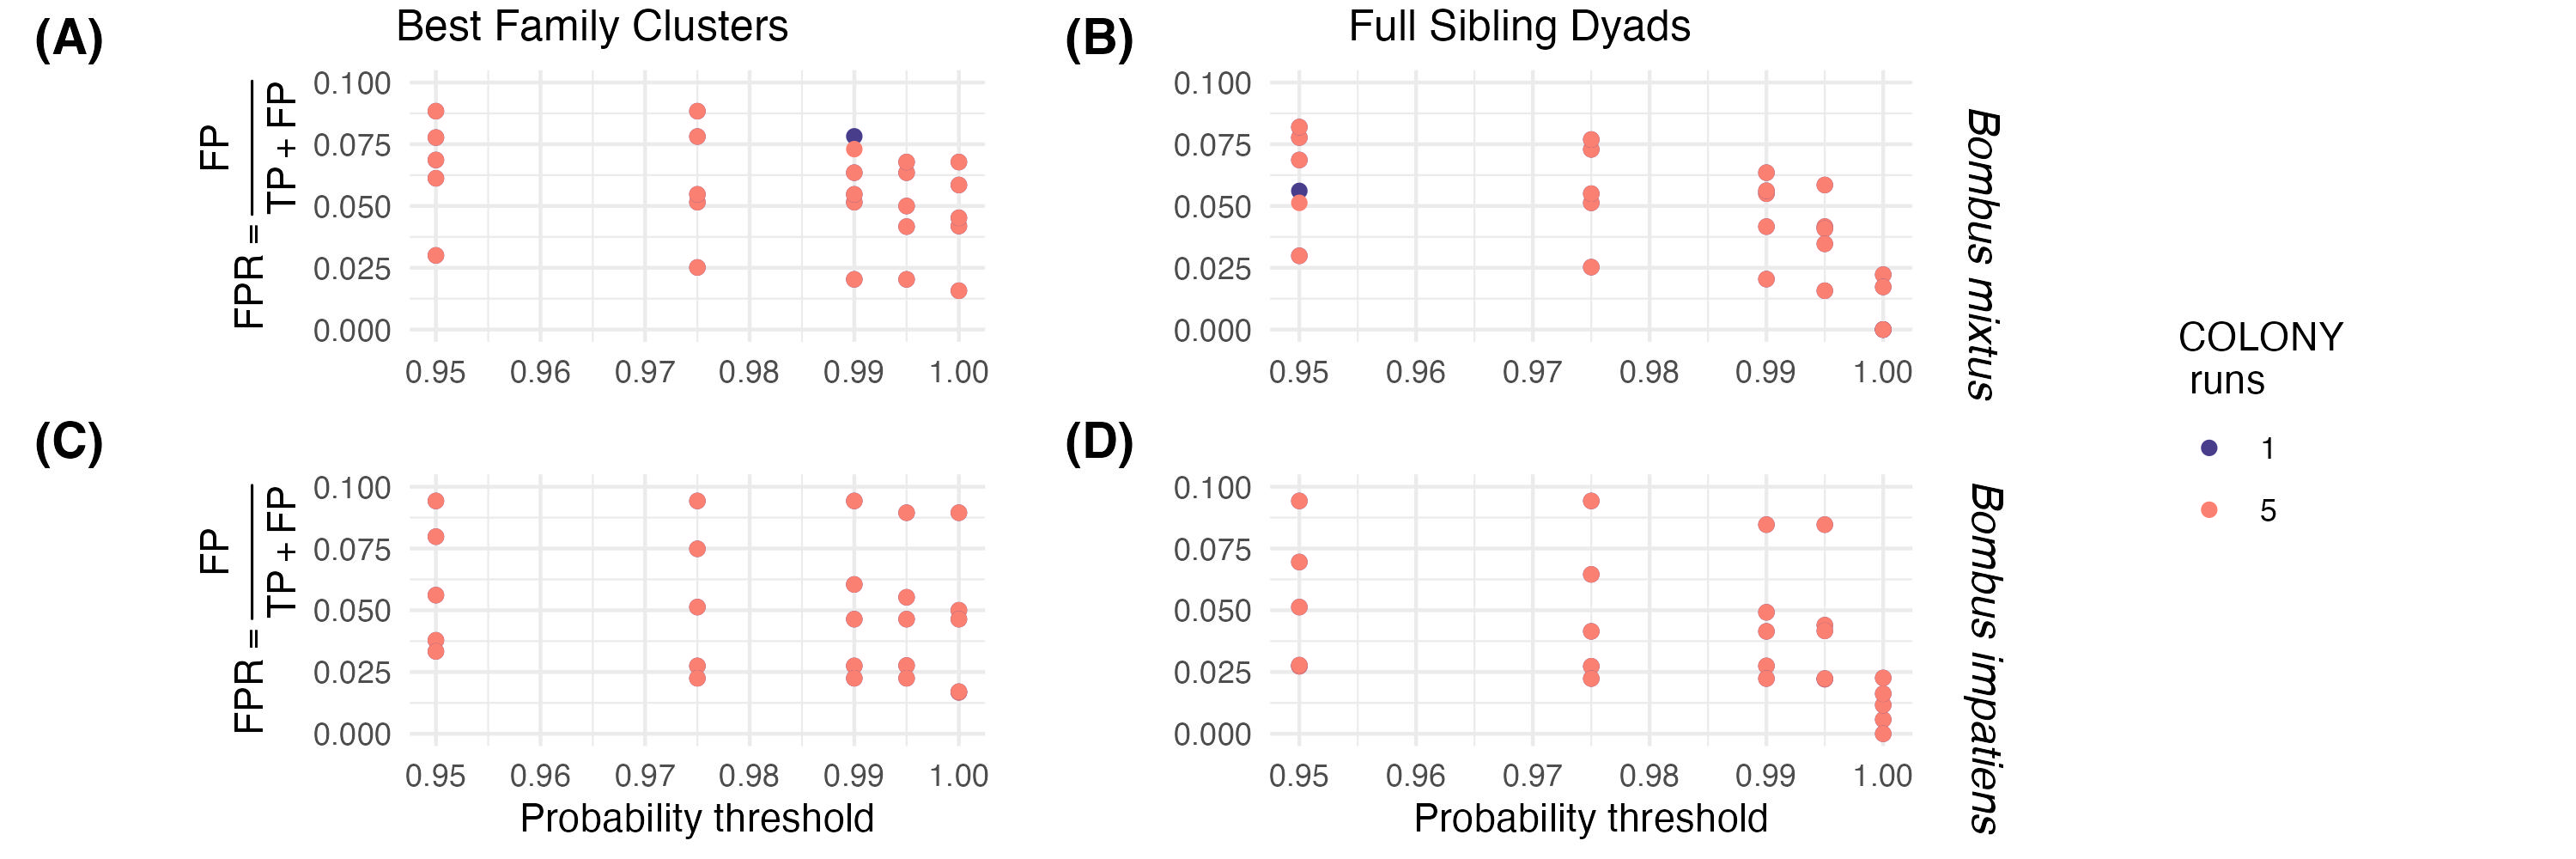
\includegraphics[width=\linewidth]{appendix_figures/fpr_repetition.jpg}
    \caption{caption}
    \label{fig:fpr_repetition}
\end{figure}

\begin{figure}[H]
    \centering
    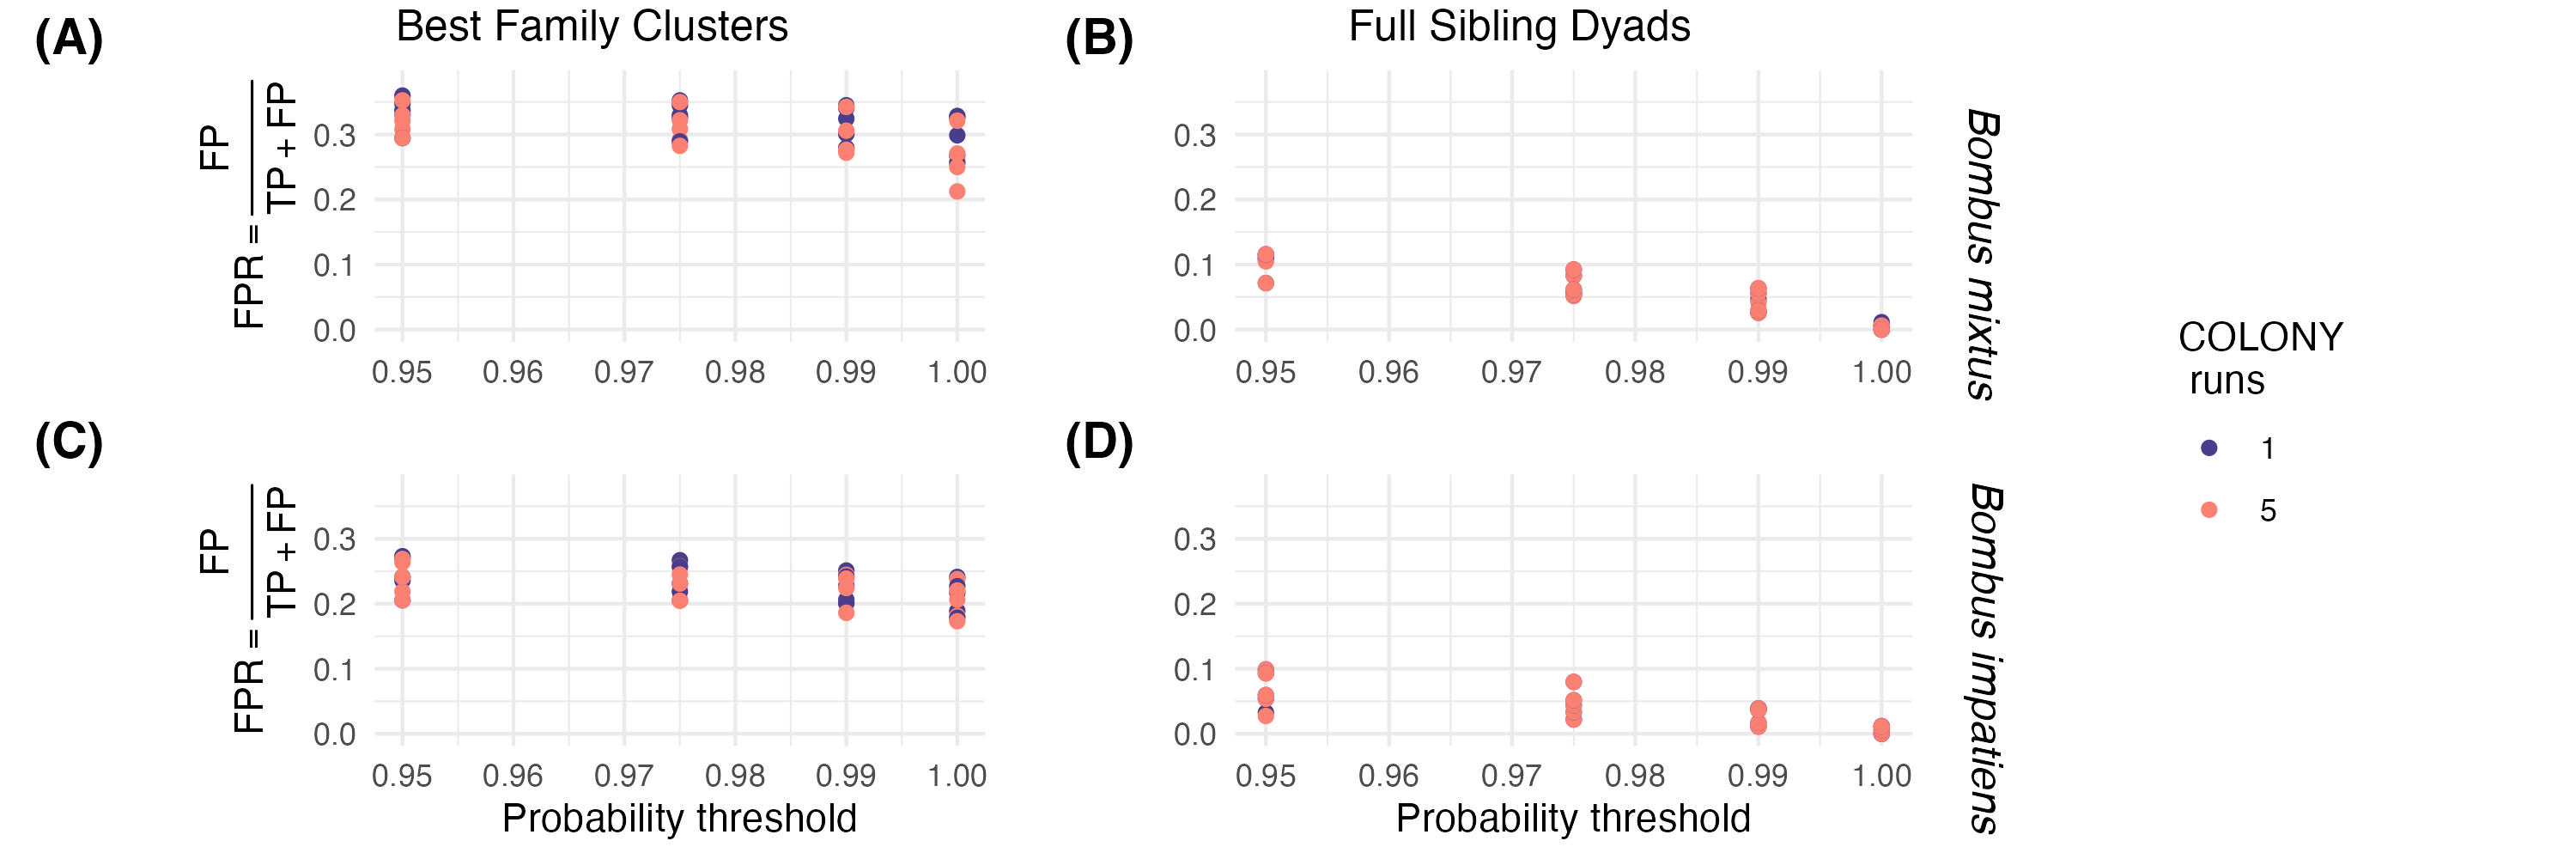
\includegraphics[width=\linewidth]{appendix_figures/fnr_repetition.jpg}
    \caption{caption}
    \label{fig:fnr_repetition}
\end{figure}

When comparing the family method to the dyad method for siblingship assignment, we found that results were strongly dependent on whether a siblingship size prior was used. The siblingship prior allows researchers to set a prior on the harmonic mean family size, based on their previous understanding of the expected family sizes in their dataset or similar datasets. Based on our preliminary analyses, when we set our siblingship prior to 1 individual per family (about 70-80\% of individuals in our true dataset were not assigned a sibling).

For this analysis, we simulated datasets of N = 2000 individuals and subsampled 20\%, 40\%, 60\%, 80\%, or 100\% of individuals to test our chosen probability threshold ($P = 0.995$) and use of siblingship priors across datasets of multiple sizes. When not utilizing a prior, we found that the family method was much less reliable than the dyad method for excluding erroneous siblingships (Fig \ref{sibprior_damilies}, data shown utilizing $P = 0.995$); false negative rates were similar for both strategies, but for the family method, 10-60\% of all inferred pairwise relationships were false positives when not using a size prior. False positive rates were consistently $\le 0.2$ when a prior was used (Fig \ref{fig:sibprior_families}). The dyad method, in contrast, resulted in $\le 12\%$ false positives for all conditions tested, and was typically $\le 5\%$ (Fig \ref{fig:sibprior_dyads}). Interestingly, we found that when we assigned siblingships based on the dyads method, the use of a siblingship size prior has little effect on the false positive or false negative rates for \emph{B. mixtus}, but caused a marginal increase in false positives and a marginal decrease in false negatives for \emph{B. impatiens} (Fig \ref{fig:sibprior_dyads}). We did not test for statistical significance, but given the qualitative results we decided to utilize the dyad method with a probability threshold of $P = 0.995$ and no siblingship size prior for our final dataset. 

\begin{figure}[H]
    \centering
    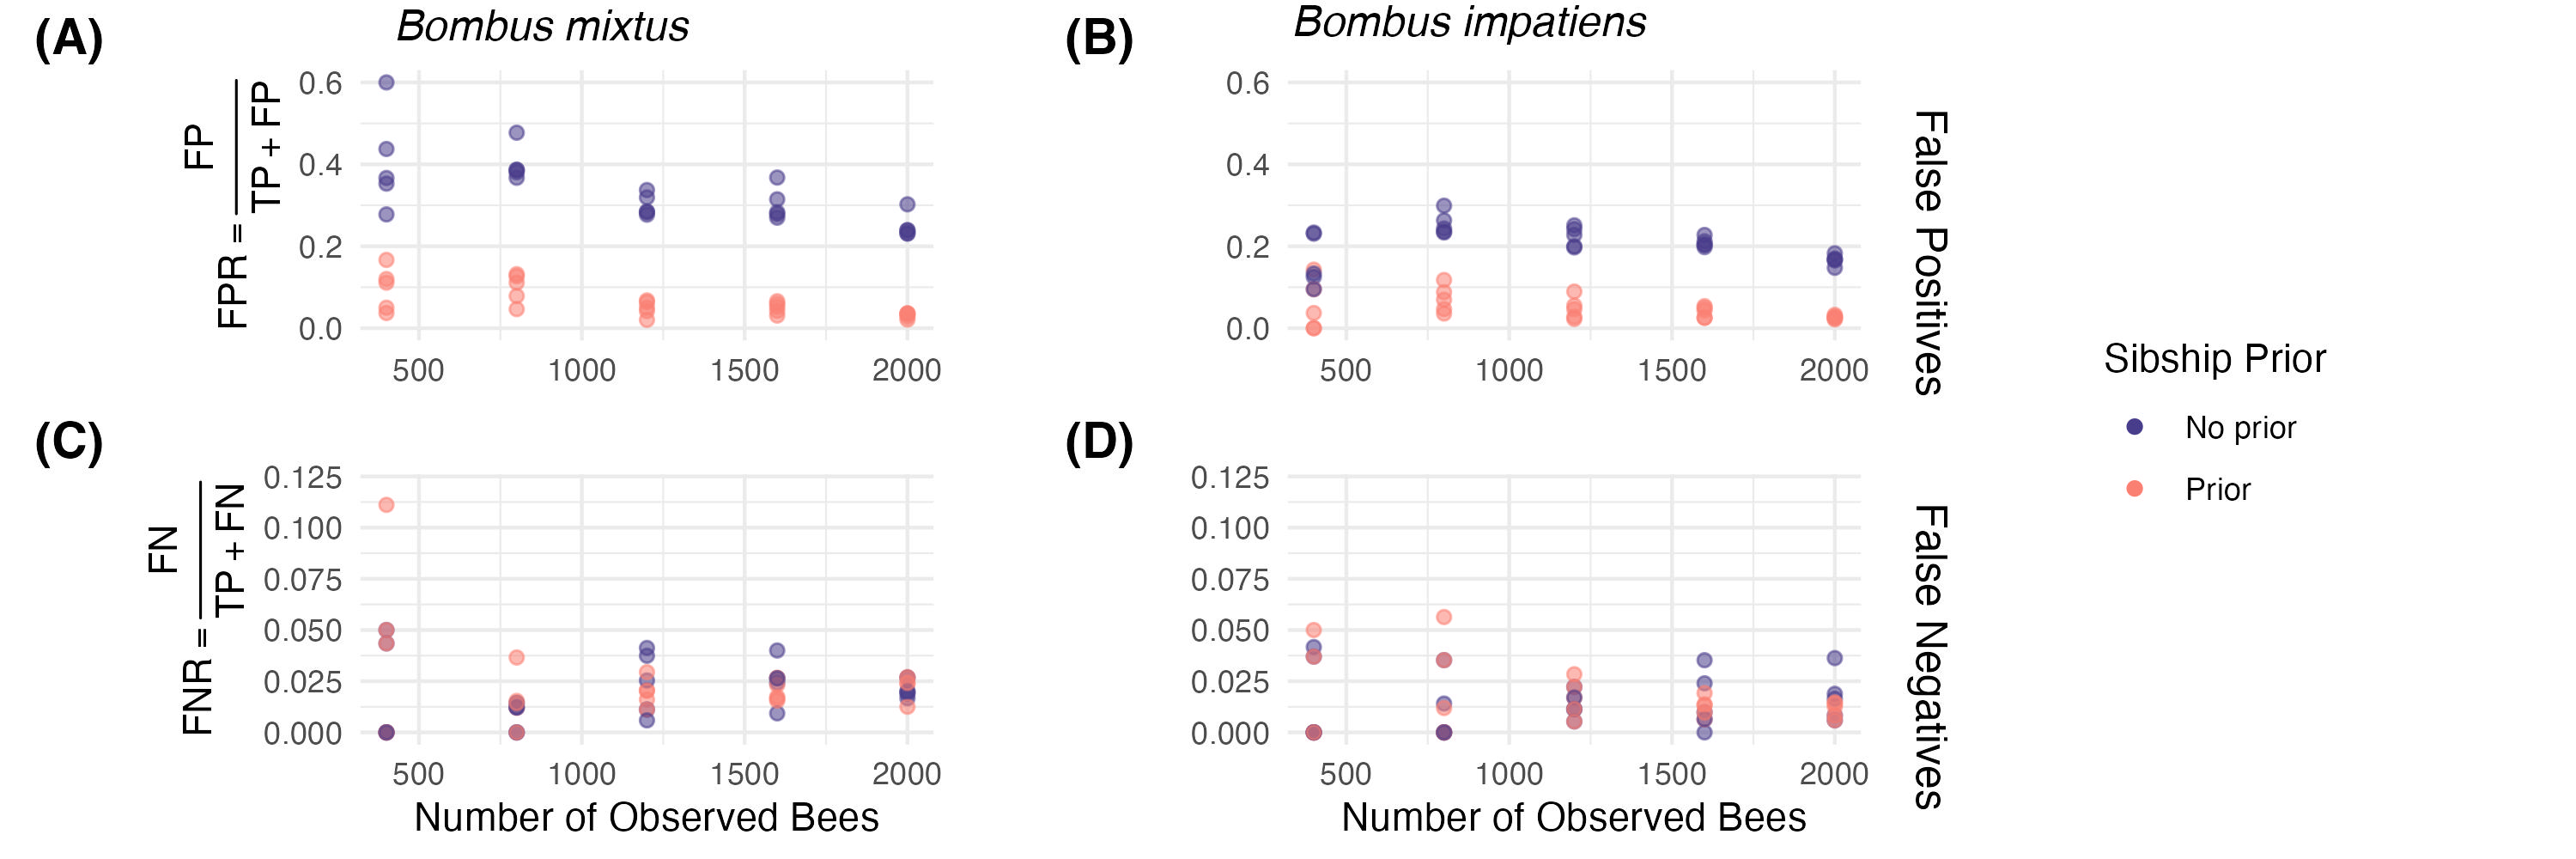
\includegraphics[width=\linewidth]{appendix_figures/sibprior_families.jpg}
    \caption{caption}
    \label{fig:sibprior_families}
\end{figure}

\begin{figure}[H]
    \centering
    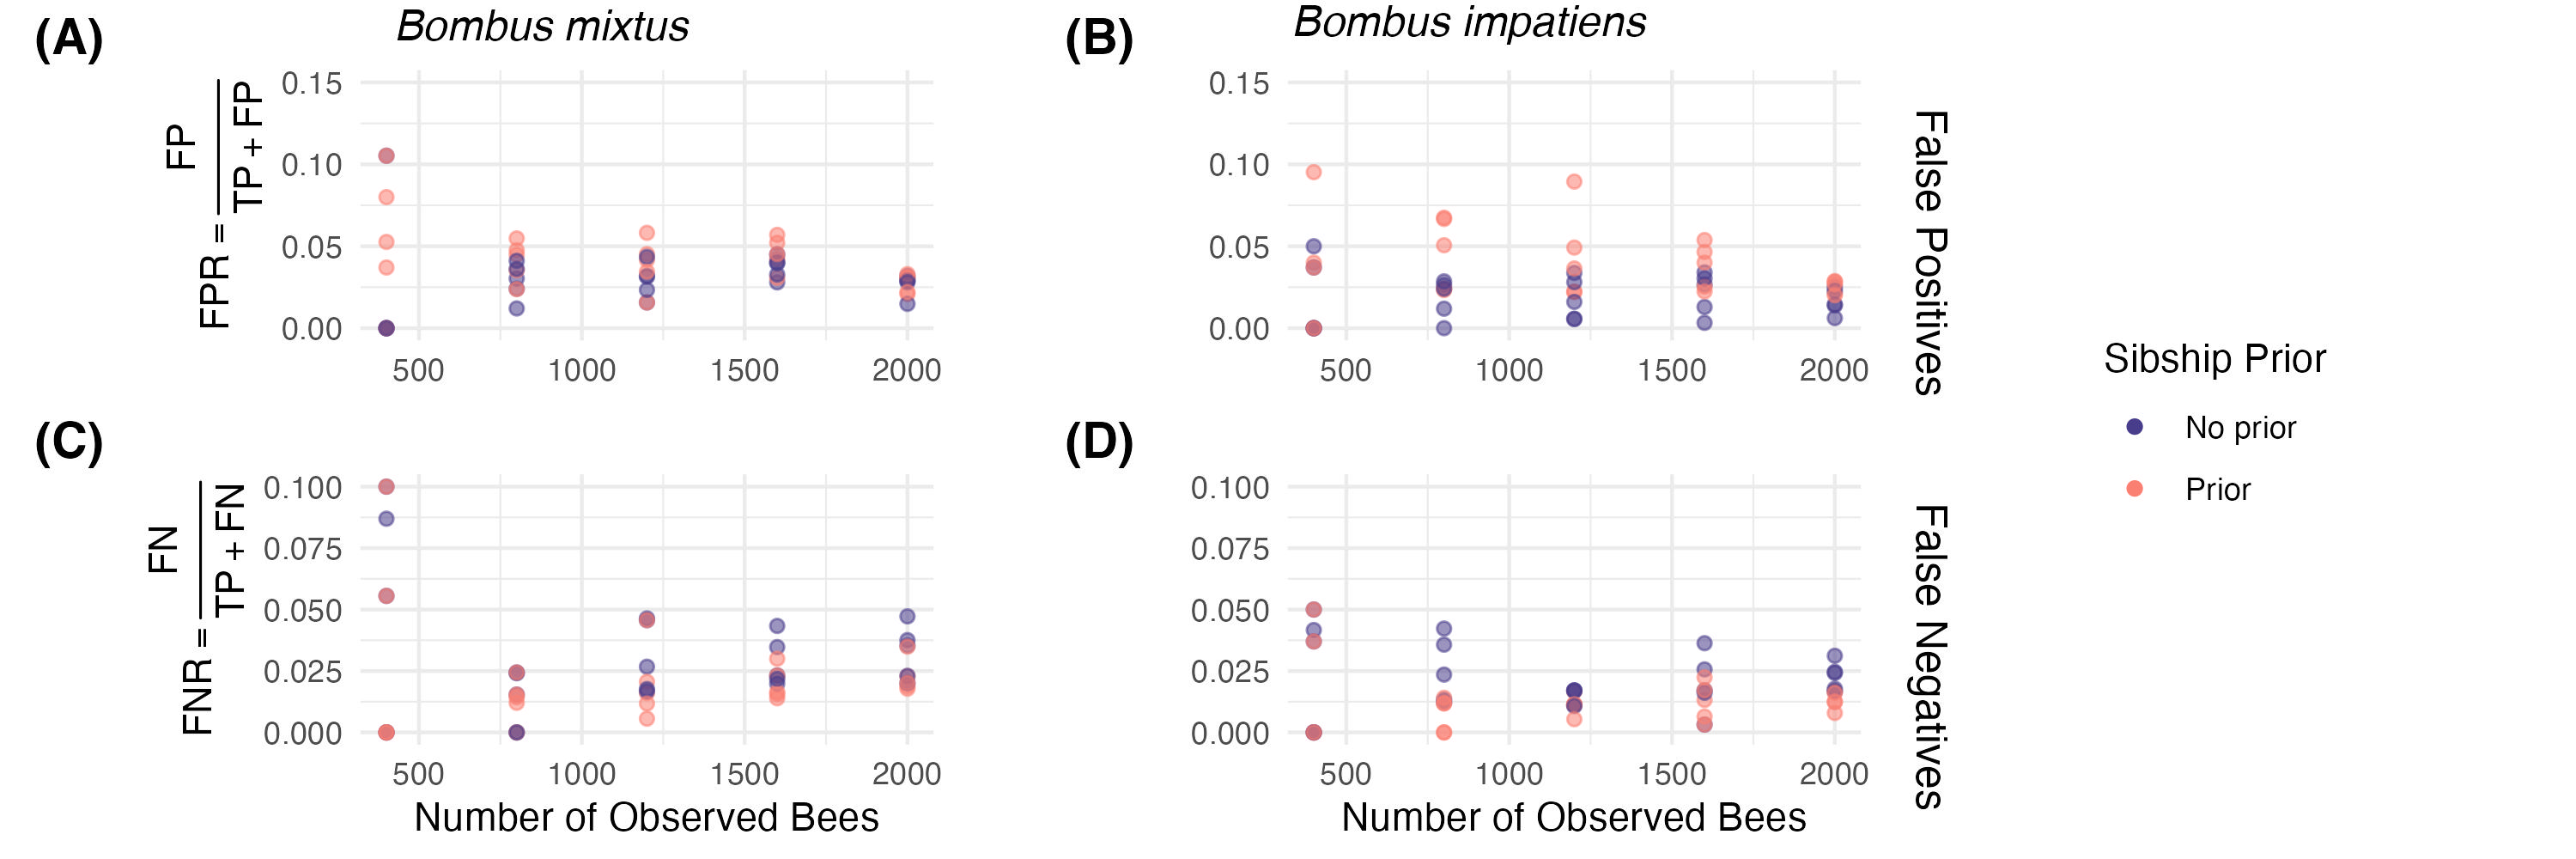
\includegraphics[width=\linewidth]{appendix_figures/sibprior_dyads.jpg}
    \caption{caption}
    \label{fig:sibprior_dyads}
\end{figure}

One benefit of using family clusters rather than sibling dyads to determine sibling relationships arises in the case of "non-circular families." These families represent cases in which some (but not all) individuals in a group are inferred to be full siblings (e.g., A related to B, B related to C, A not related to C). Such cases are rare, but are handled internally by COLONY such that all inferred family clusters are circular. Because we choose here to refer to dyad pairs rather than family clusters, we are left the task of deciding how to resolve non-circular families---indeed, resolution of non-circular families could be one process which leads to a higher false positive rate.

Because of this uncertainty, we explored several heuristics for resolving non-circular families. We started by exploring the structure of non-circular families in our simulated datasets, to determine whether non-circularity is more frequently the result of false positives (e.g., a third individual being erroneously added to a sibling pair) or false negatives (e.g., failure to detect a sibling relationship between any pair of siblings in a triad).

To do this, we plotted non-circular families from all five simulations, using a threshold of $P = 0.99$ for inclusion of pairwise relationships.

%% PLOT NON CIRCULAR FAMILIES AND EXPLORE HEURISTICS FOR DEALING WITH THEM
b

\subsection{Assessing the use of cross-site sibling exclusion for reducing false positive rates}

We next systematically evaluated the use of sibling exclusion criteria and siblingship size priors to determine whether these software specifications have any impact on siblingship inference accuracy. Previous studies on \emph{Bombus} have varied in their approaches to the scale at which possible siblingships are evaluated, with some studies performing separate runs of the software for populations sampled at different sites/regions (CITE: JHA? ) while others group populations at larger scales, permitting the discovery of long distance foraging or dispersal events between sites (CITE: LEPAIS, MOLA, ETC. RAO?). While identifying the maximum foraging or dispersal range for different species or landscape contexts is an important goal, we consider two challenges to this method, related to (i) the rarity of capturing individuals engaged in such long distance events, and (ii) the statistical challenges introduced by a very high number of pairwise comparisons between individuals at different sites. For a more thorough discussion of the first point, we direct the reader to \textcite{lepaisEstimationBumblebeeQueen2010a}. Ultimately, we posit that the rate at which such events should be captured is much lower than both the false positive and false negative rates of the COLONY software, due to the quadratically increasing search area over which foragers will be dispersed as distance from their nest increases (see discussion in \textcite{osborneBumblebeeFlightDistances2008}). Furthermore, given the large sample sizes of our populations, and the fact that the majority of pairwise comparisons (without exclusion) will occur between individuals at different sites, we hypothesized that allowing for siblingship assignments between all individuals would result in a high percentage of false positive relationships that would severely bias estimates of colony locations and foraging behaviour.

To test this hypothesis, and to determine whether total sample size had an effect on the utility of excluding cross-site siblingships, we simulated five datasets of n = 2000 individuals, and subsetted each data set to contain 20, 40, 60, 80, or 100\% of the initial samples. These data were simulated to reflect trapping grids which were arranged in a 3 x 2 grid with traps in adjacent grids at least 6km apart. The minimum distance between adjacent trapping grids in our real data was 5km (also separated by a large river, expected to limit dispersal), and all other sites were at least 7km apart. The mean foraging distance of colonies in our simulation was set to 1km (99\% of all visitations within 3.32km). This would allow for colonies located midway between trapping grids to sampled at two sites, while reflecting the fact that the majority of bumblebee foraging is thought to occur within (at \emph{most}) a few kilometers of the nest. We therefore believe that the simulated data would represent a relatively optimistic view of the number of cross-site siblingships which could be present in the real data.

We created siblingship exclusion tables for COLONY by excluding (for each individual) all potential siblingships with individuals captured at different trapping grids (sites). We ran COLONY on each dataset with and without incorporation of the siblingship exclusion table. Further software specifications for these runs can be found in Table \ref{tab:softwarespecs}. We used the dyad method and an exclusion threshold of $P = 0.99$ as described in the previous subsection.

We found that for both species (\emph{B. mixtus} and \emph{B. impatiens}) and for all tested sample sizes (n = 400-2000 individuals), cross-site sibling exclusion resulted in a lower false positive rate (Fig \ref{fig:excl_size} A-B). The variation in false positive rates between independent simulations decreased with increasing sample size. When using cross-site exclusion, mean false positive rates were fairly consistent across sample sizes, but without cross-site exclusion, the mean false positive rate tended to decrease with increasing sample size.

False negative rates were similar for both methods, indicating that cross-site exclusion did not cause us to lose a high proportion of real cross-site siblingships (Fig \ref{fig:excl_size} C-D). Indeed, manual inspection of datasets revealed that cross-site sampling was extremely rare or non-existant, given our parameterization and sample size.

\begin{figure}[H]
    \centering
    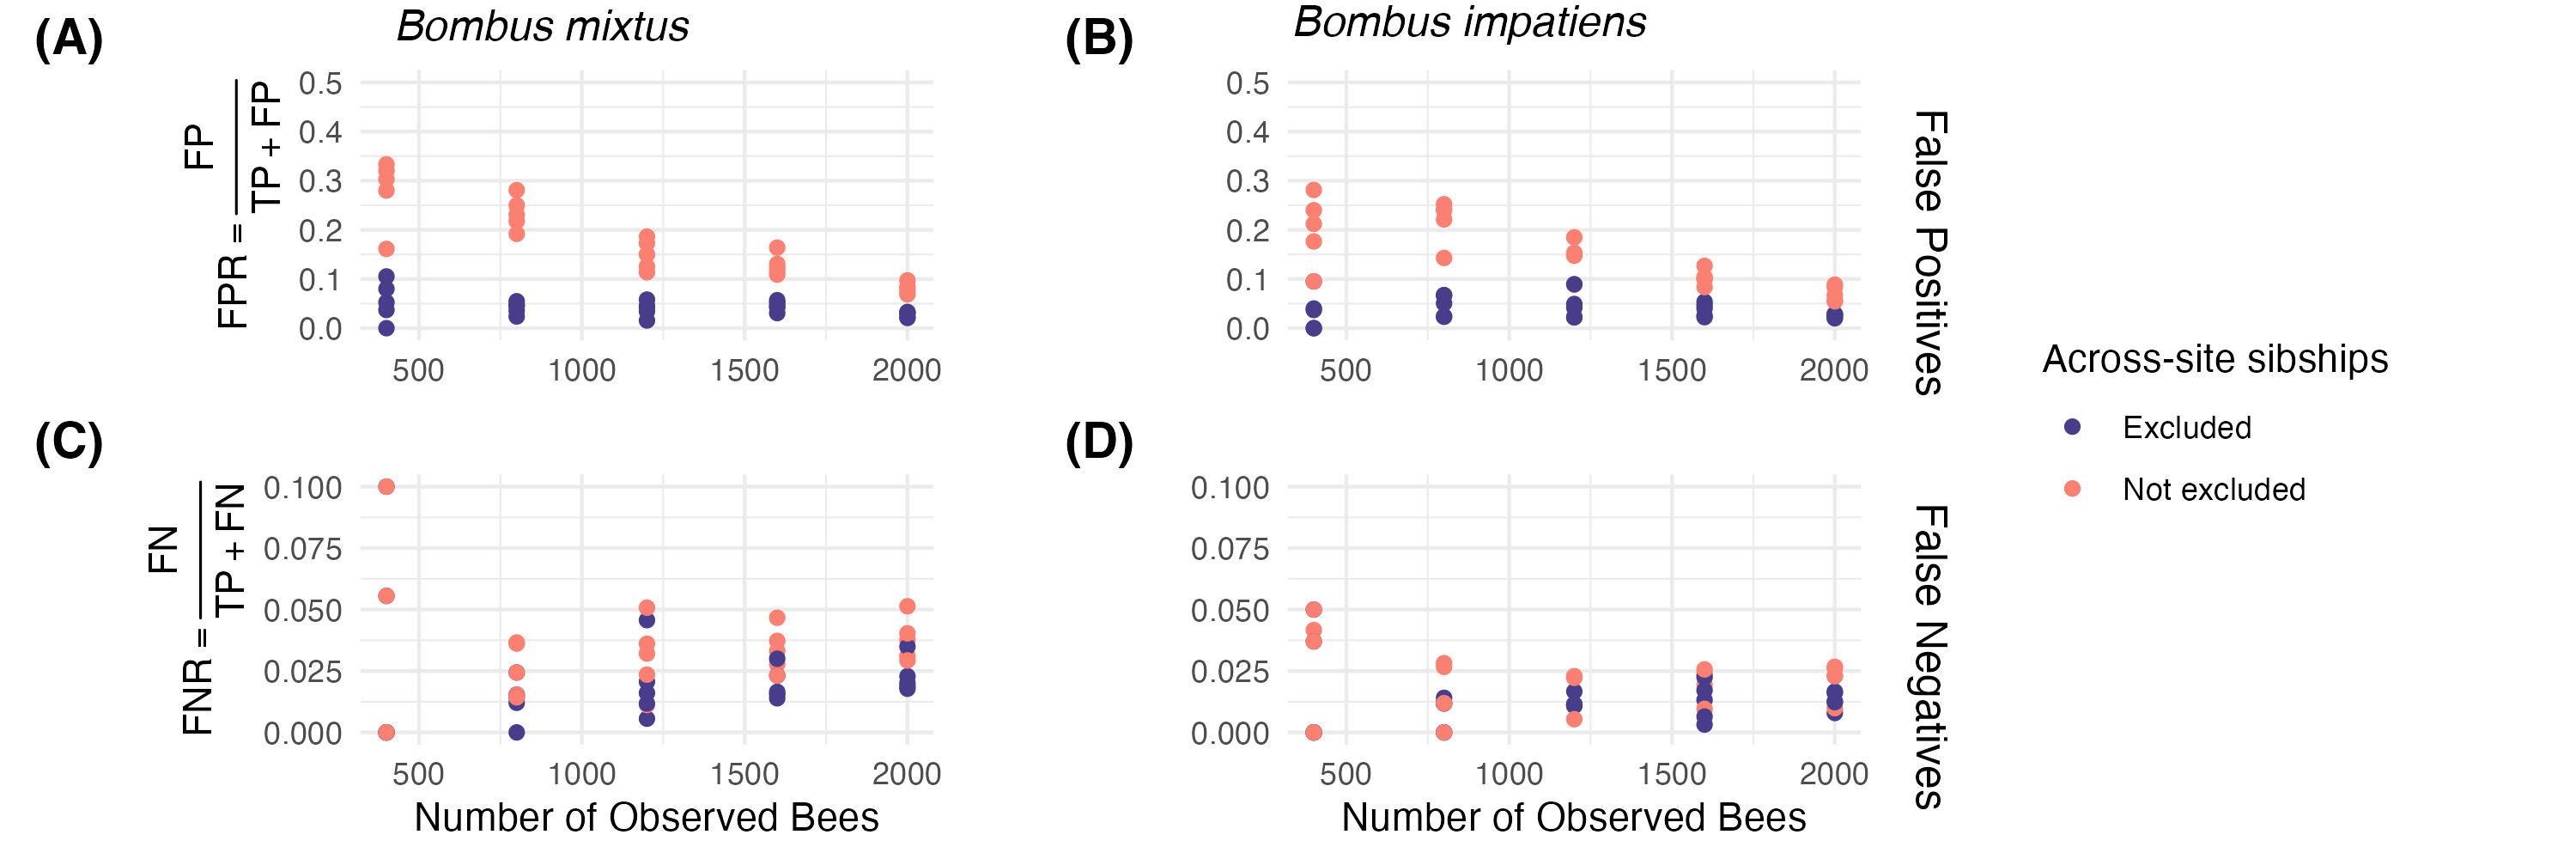
\includegraphics[width=\linewidth]{appendix_figures/excl_size.jpg}
    \caption{caption}
    \label{fig:excl_size}
\end{figure}


\subsection{Evaluating the effects of multiple paternity on siblingship inference}
% Multiple paternity results

\begin{table}
\centering
\caption{Description of software settings (COLONY 2.0.6.5 \parencite{jonesCOLONYProgramParentage2010}) for simulations.}
\label{tab:simulationspecs}
\footnotesize
\begin{tabular}{ p{2cm}  p{3.5cm} p{2cm} p{2.5cm} p{2cm} p{1.5cm}}
\hline
\textbf{Simulation}& \textbf{Comparison}&\textbf{Sample Size}& \textbf{Sibship Size Prior}& \textbf{Cross-site Exclusion}& \textbf{Runs}\\
\hline
\textbf{Subsection 1} & Number of COLONY runs& 1200 & yes& yes& 1-5 \\
\hline
\textbf{Subsection 1} & Probability threshold& 1200 & yes & yes & 1-5  \\
\hline
\textbf{Subsection 1} & Families vs dyads & 1200 & yes& yes& 1-5\\
\hline
\textbf{Subsection 2} & Siblingship size prior & 400-2000 & yes/no & yes/no& 1 \\
\hline
\textbf{Subsection 2} & Cross-site exclusion & 400-2000 & yes/no & yes/no& 1\\
\hline
\textbf{Subsection 3} & Mating system& 1000 & no & no& 1 \\
   \hline  
\textbf{Subsection 3} & Mating system (augmented data)& 1000 & yes & no& 1 \\
   \hline  
\end{tabular}
\end{table}





\section{Observing colonymates at multiple sites}


\end{document}